\section{Selective Attention Memory Network (SAMNet)}

%\begin{figure}[!b]
%\begin{minipage}{0.43\textwidth}
%	\centering
%	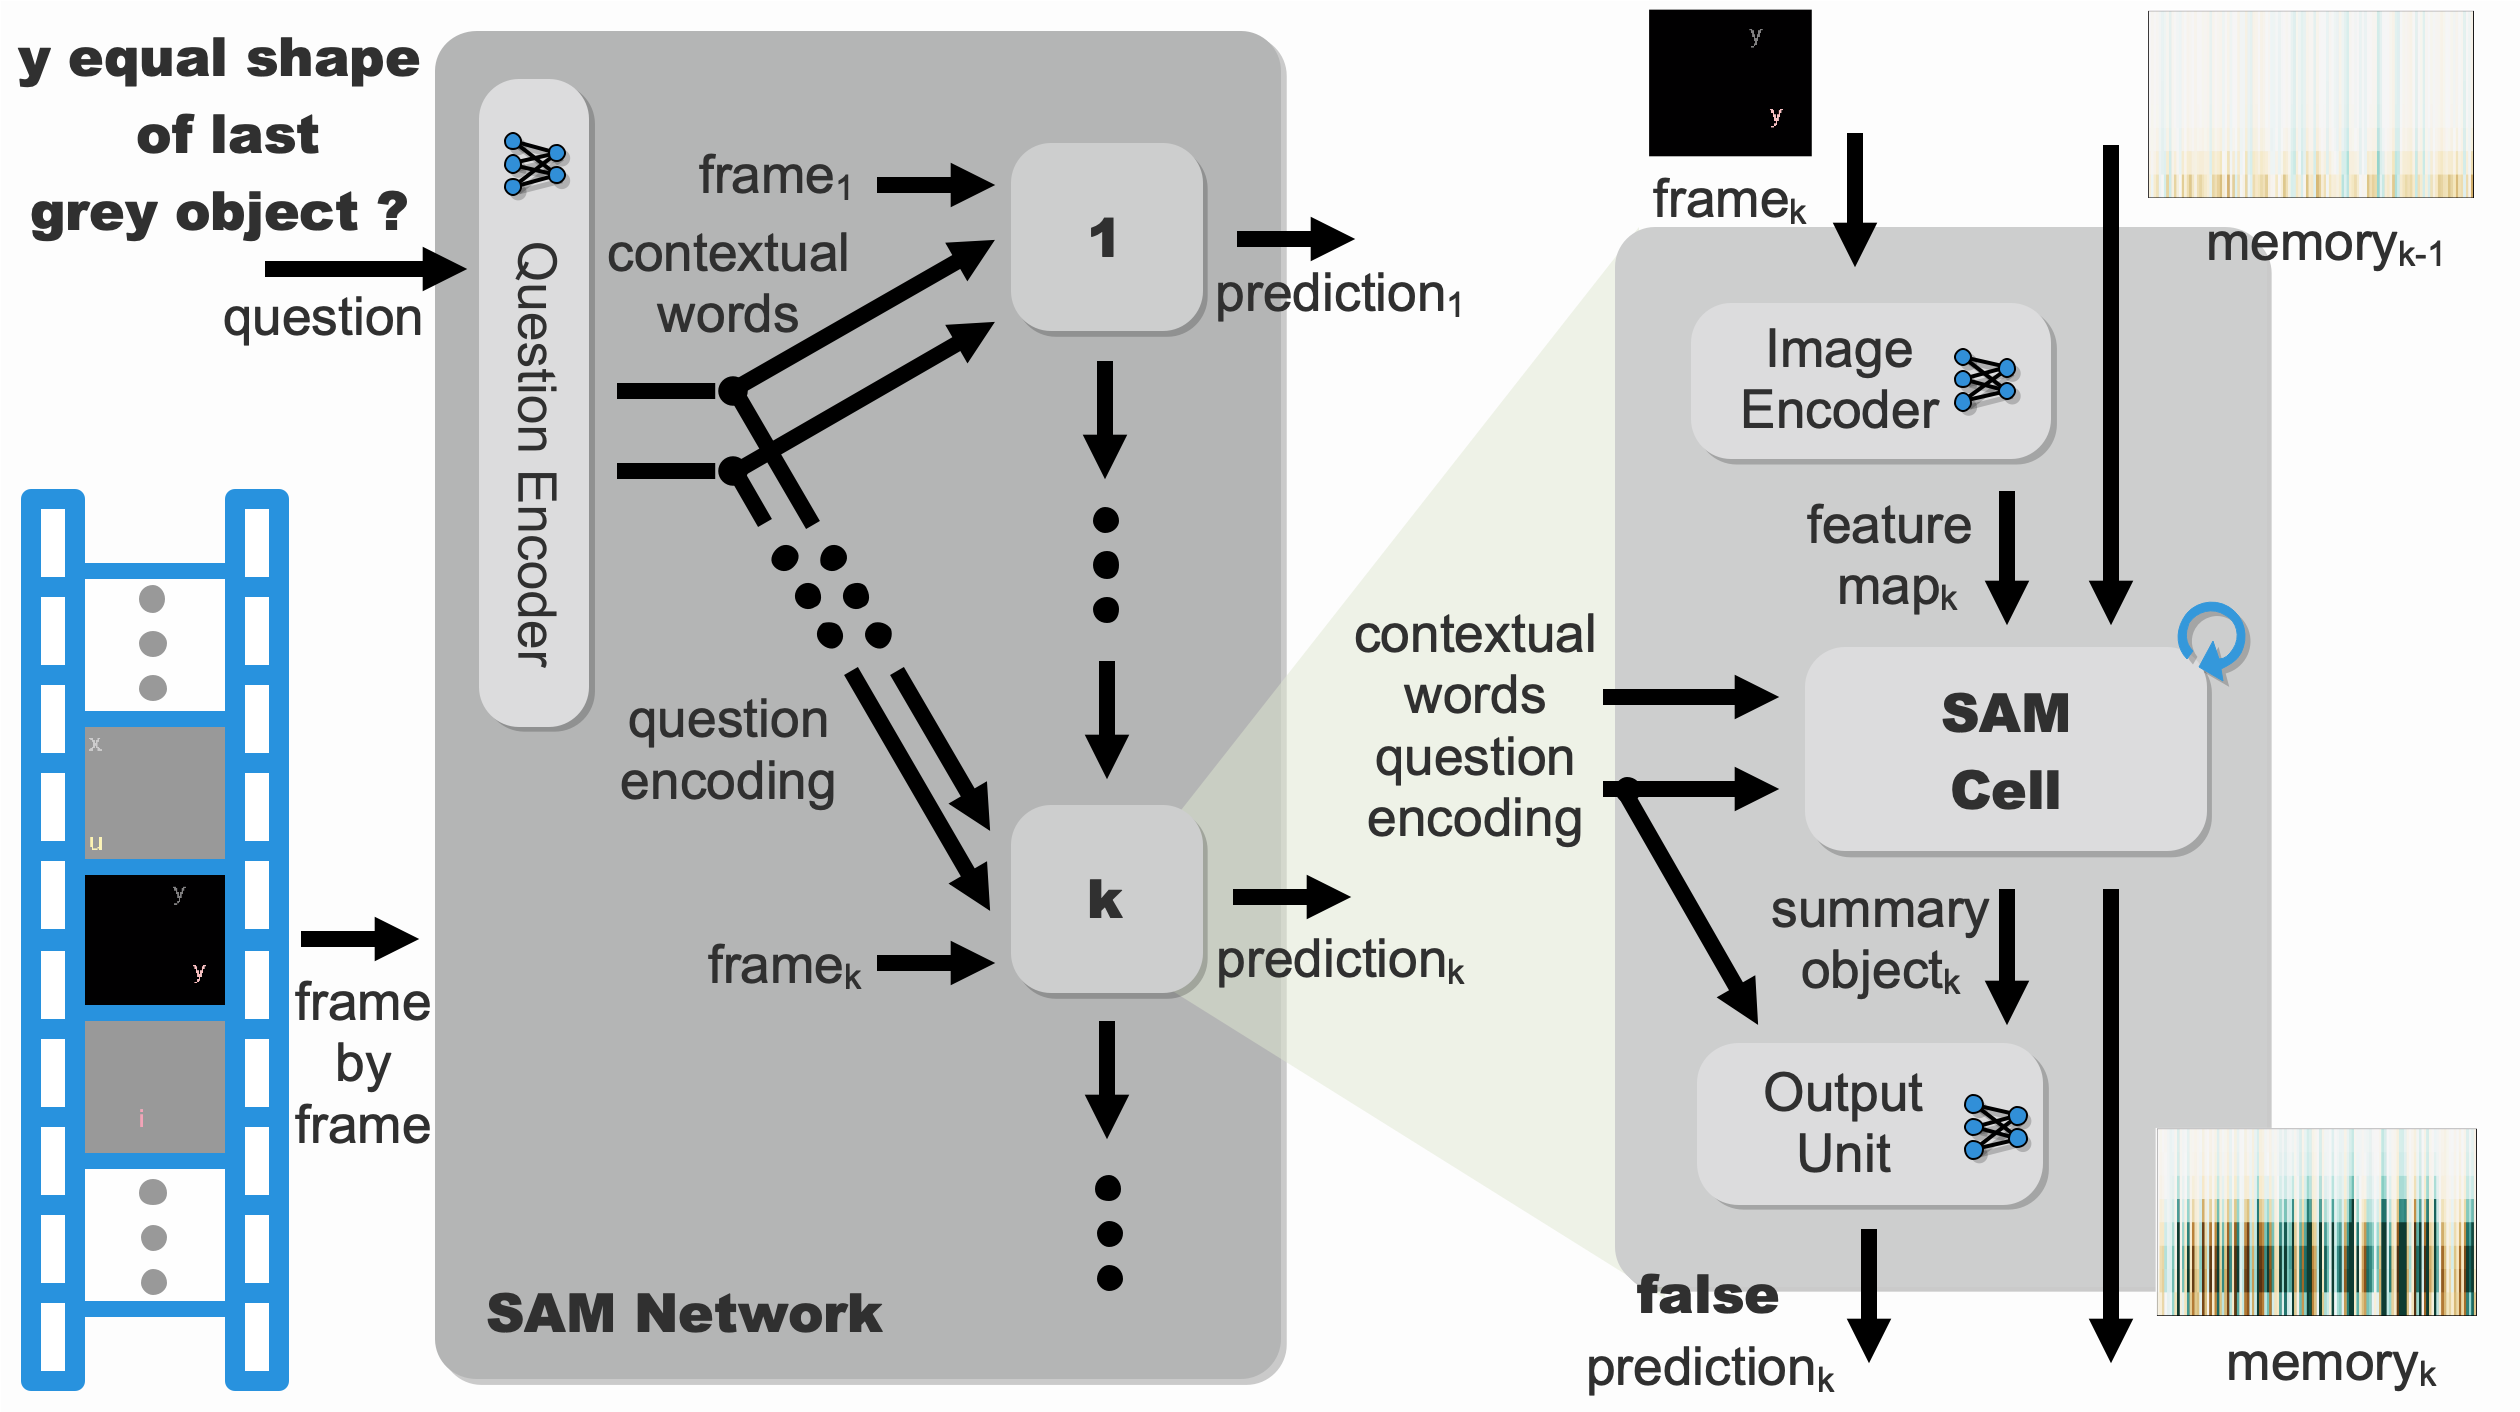
\includegraphics[width=\textwidth]{../img/architecture/samnet_architecture4}
%\end{minipage}\hfill
%\begin{minipage}{0.55\textwidth}
%	\centering
%	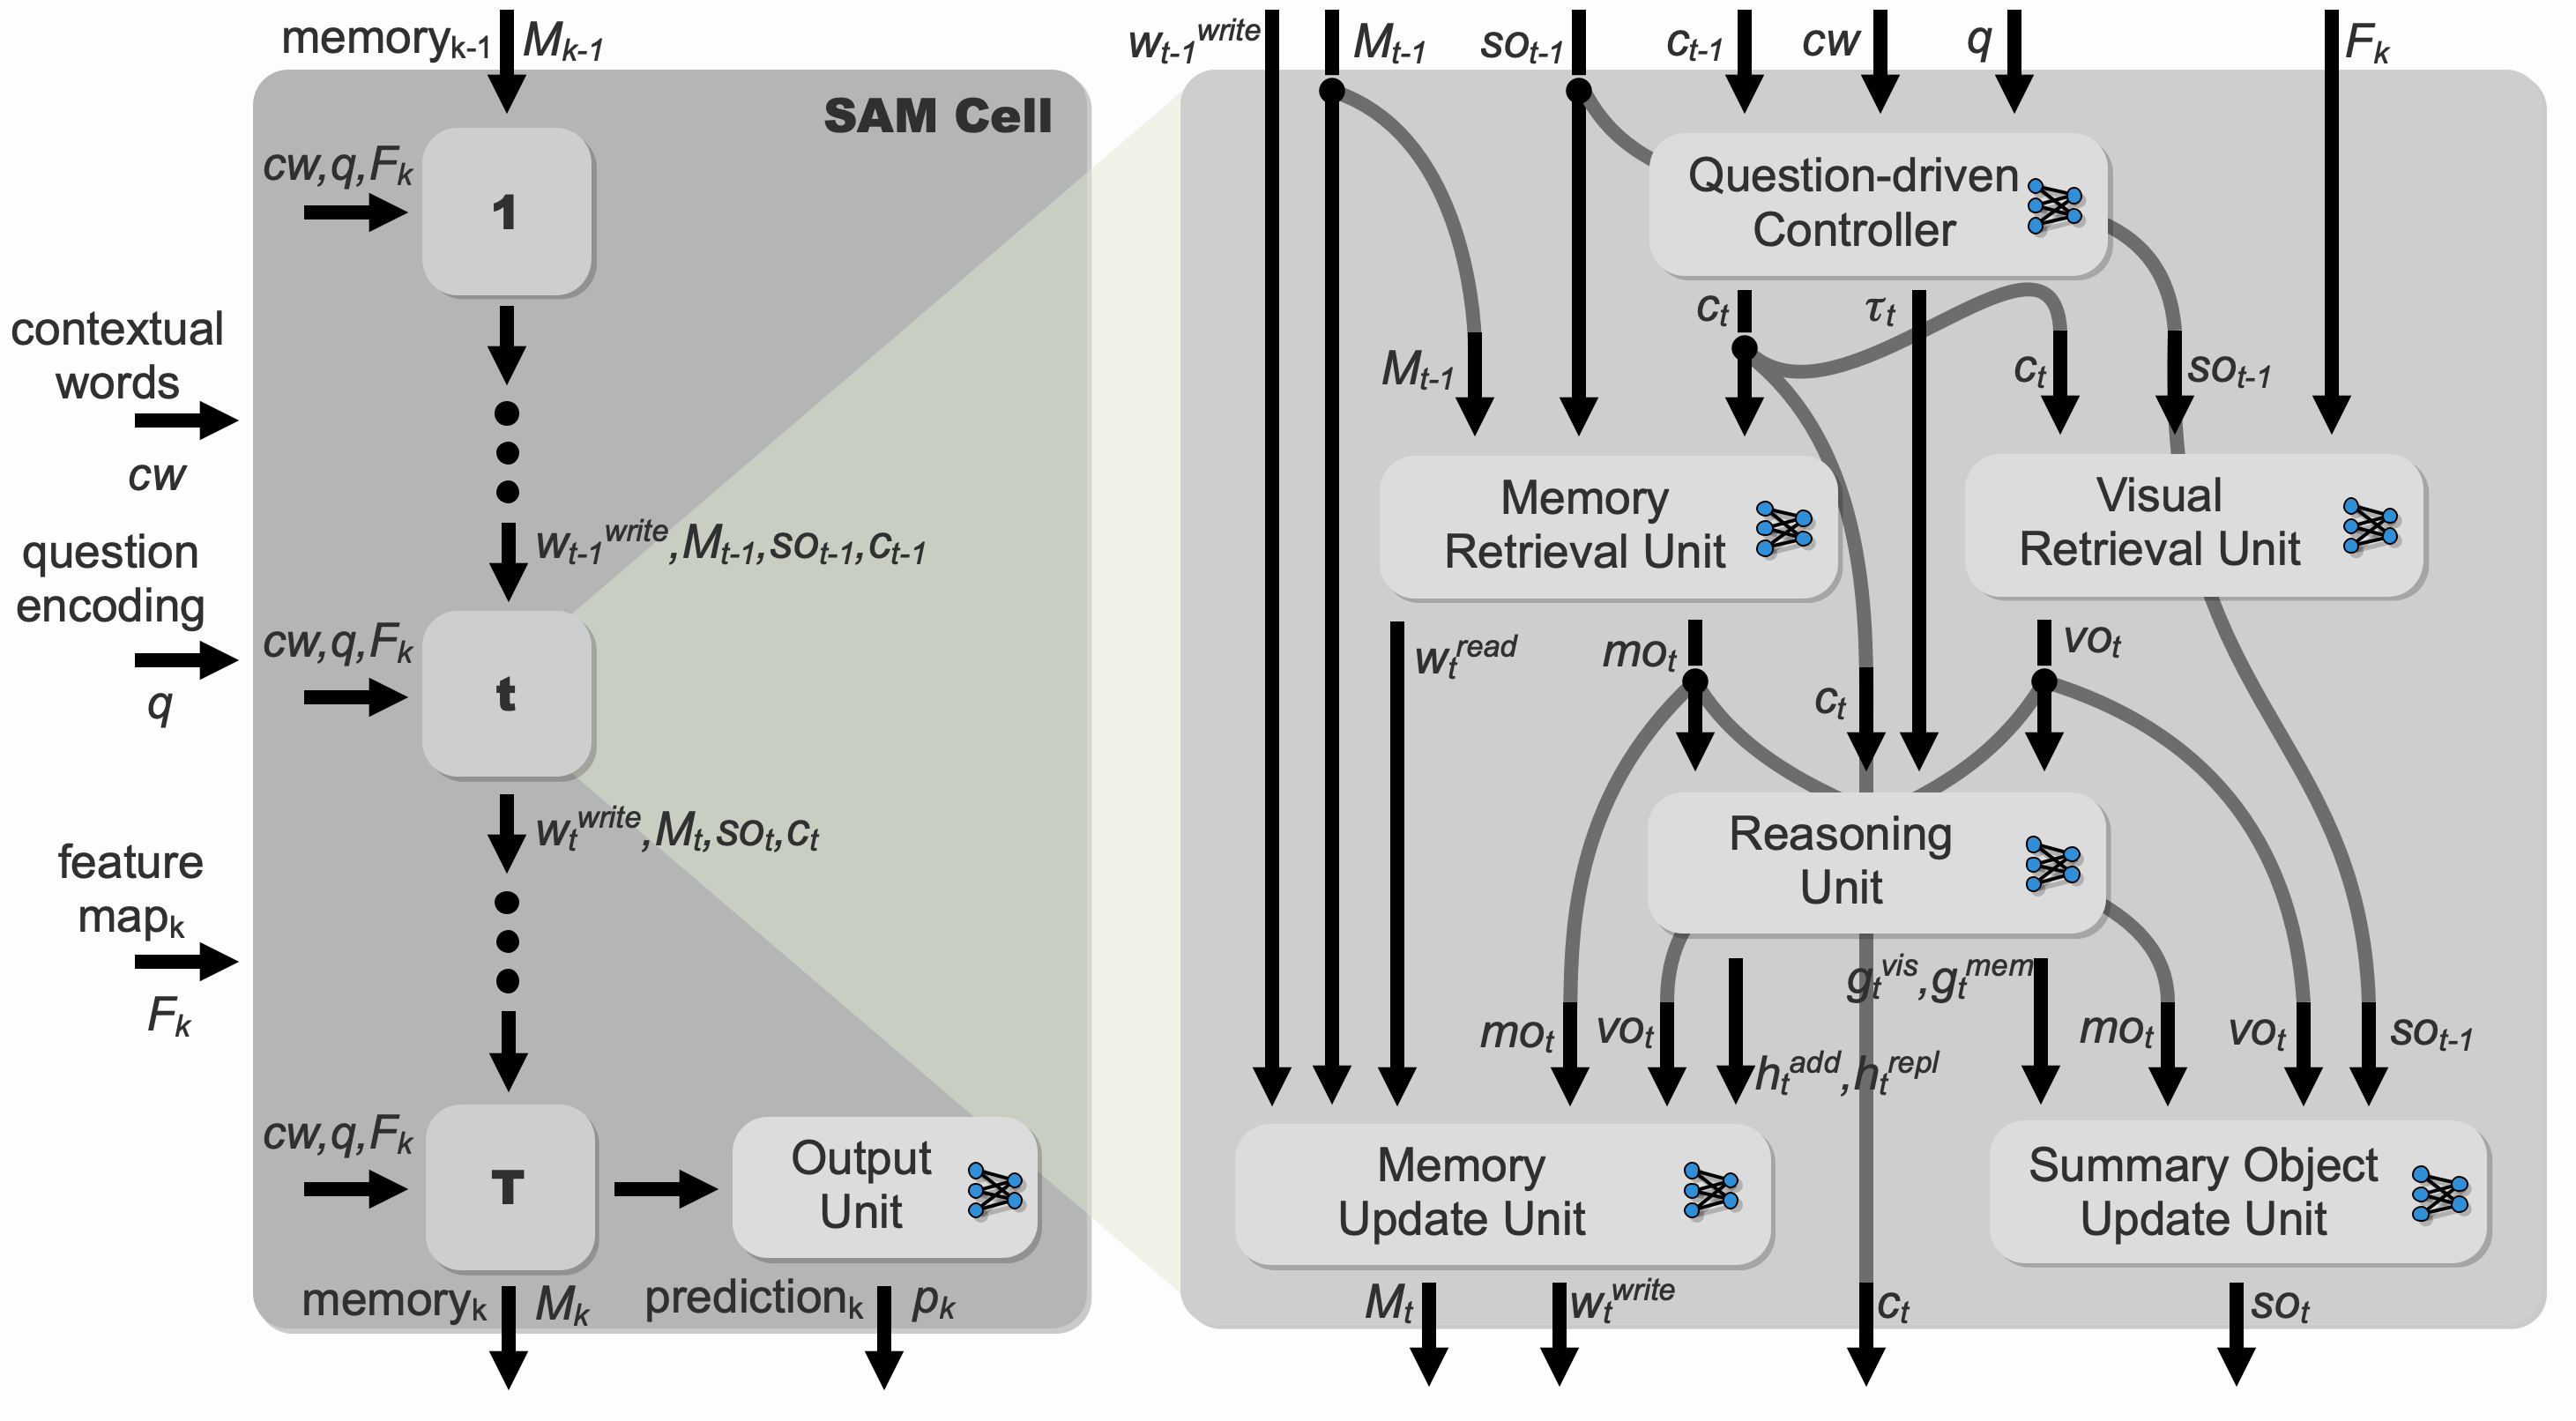
\includegraphics[width=\textwidth]{../img/architecture/samcell_reasoning}
%\end{minipage}\hfill
%\caption{General architecture of SAMNet (left) and a single reasoning step in SAMCell (right)}
%\label{fig:samnet}
%\end{figure}	

%Selective Attention Memory Network (SAMNet) is a end-to-end differentiable model made for video reasoning. It is a model based on attention mechanisms but also on a Selective Attention Memory which is able to store selected entities. This memory enables SAMNet to reason across multiple frames and perform spatio-temporal reasoning. 
%The core of SAMNet is based a recurrent cell called SAMCell. By aligning together a series of k SAMCells per frame, the network can perform k reasoning steps over a frame. At every new frame, a new series of k SAMCells is initiated. The SAMCell can read and write to memory at every frame using a content addressable mechanism. This section describes the model and the different units that composed a SAMCell. They are called the Question-driven Controller, the Visual Retrieval Unit, the Memory Retrieval Unit, the Reasoning unit, the Memory update unit, and the Summary Object Udpate Unit. 
%The model is also composed of an Image Encoder and a Question Encoder both responsible to pre-process the visual and textual inputs. The output unit is a classifier.
%All those modules are described below.

\begin{figure}[hbtp]
	\centering
	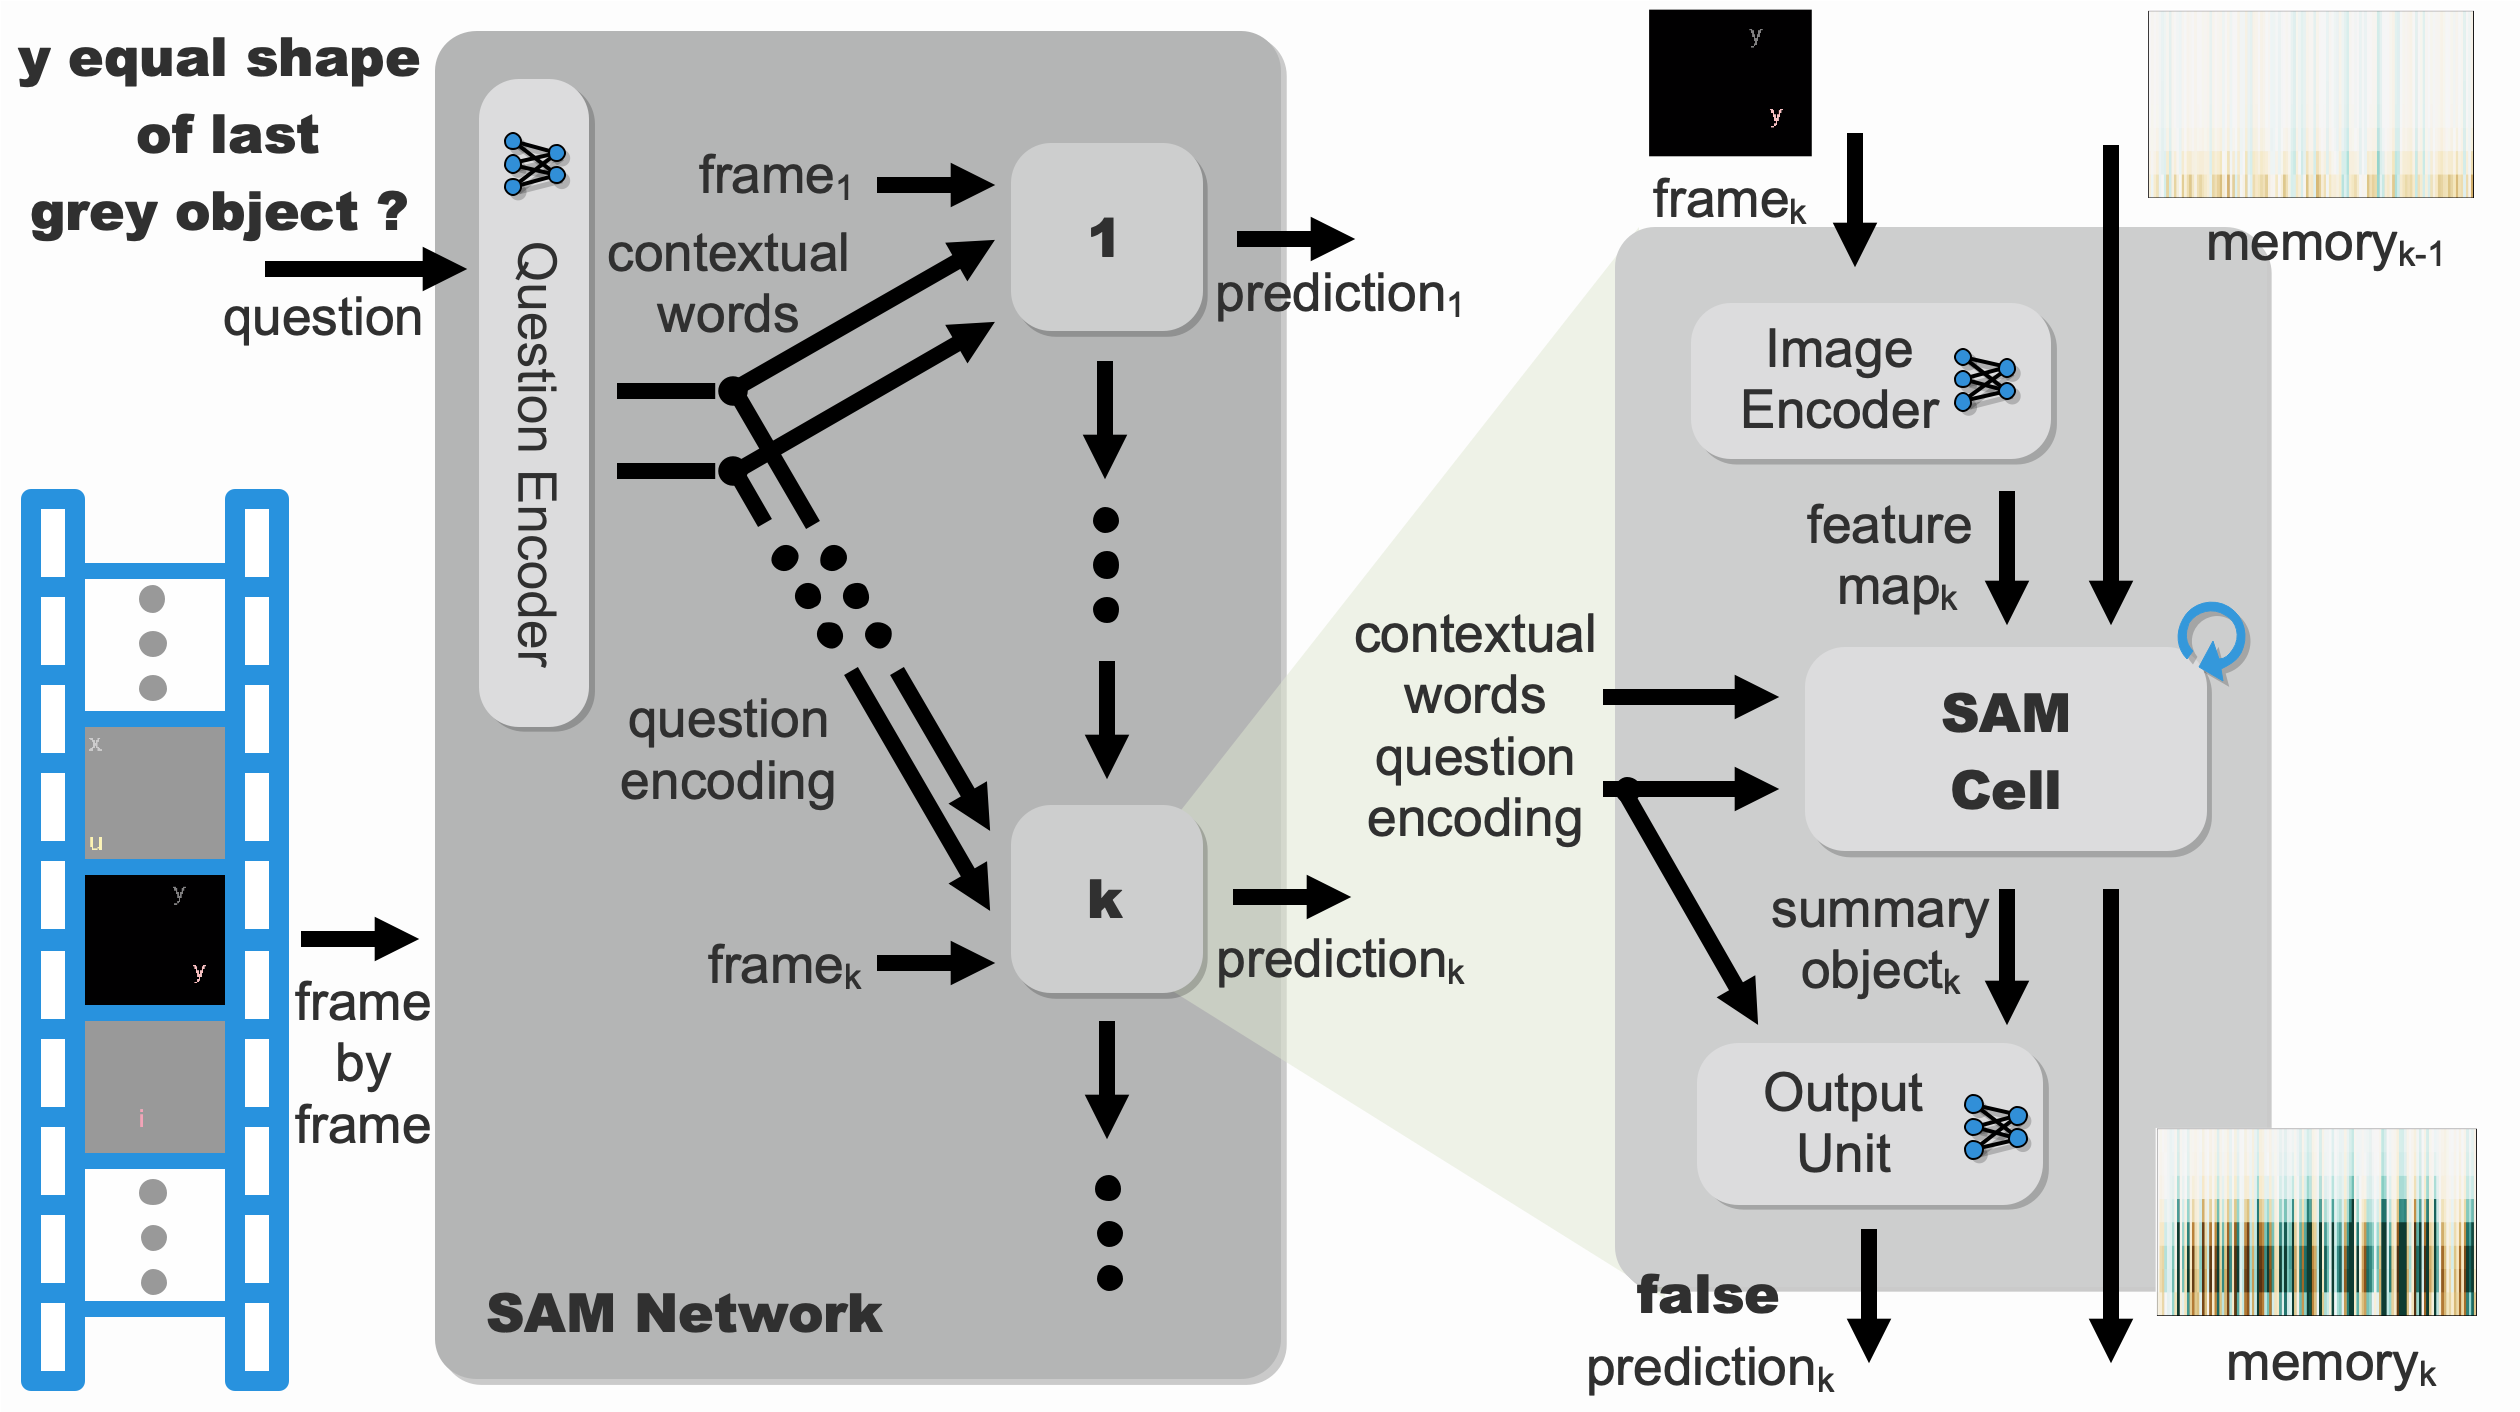
\includegraphics[width=\textwidth]{../img/architecture/samnet_architecture4}
	\caption{General architecture of SAMNet}
	\label{fig:samnet}
\end{figure}	

SAMNet is an end-to-end differentiable recurrent model equipped with an external memory for enabling multi-step reasoning over text and video (\cref{fig:samnet}).
The memory is used to store relevant objects representing contextual information about words in text and visual objects in video frames. 
Each address of the memory stores a $d$-dimensional vector, where $d$ is a global parameter.
The memory  can be accessed through either content-addressing, via dot-product attention, or location-based addressing. 
Coupled with gating mechanisms to be described later, this enables correct objects to be retrieved 
in order to perform spatio-temporal reasoning on frames and text. 
%A notable feature of this design is that the number of addresses $N$ can be set to different values during training and 
%testing to fit the characteristics of data.

\begin{figure}[hbtp]
	\centering
	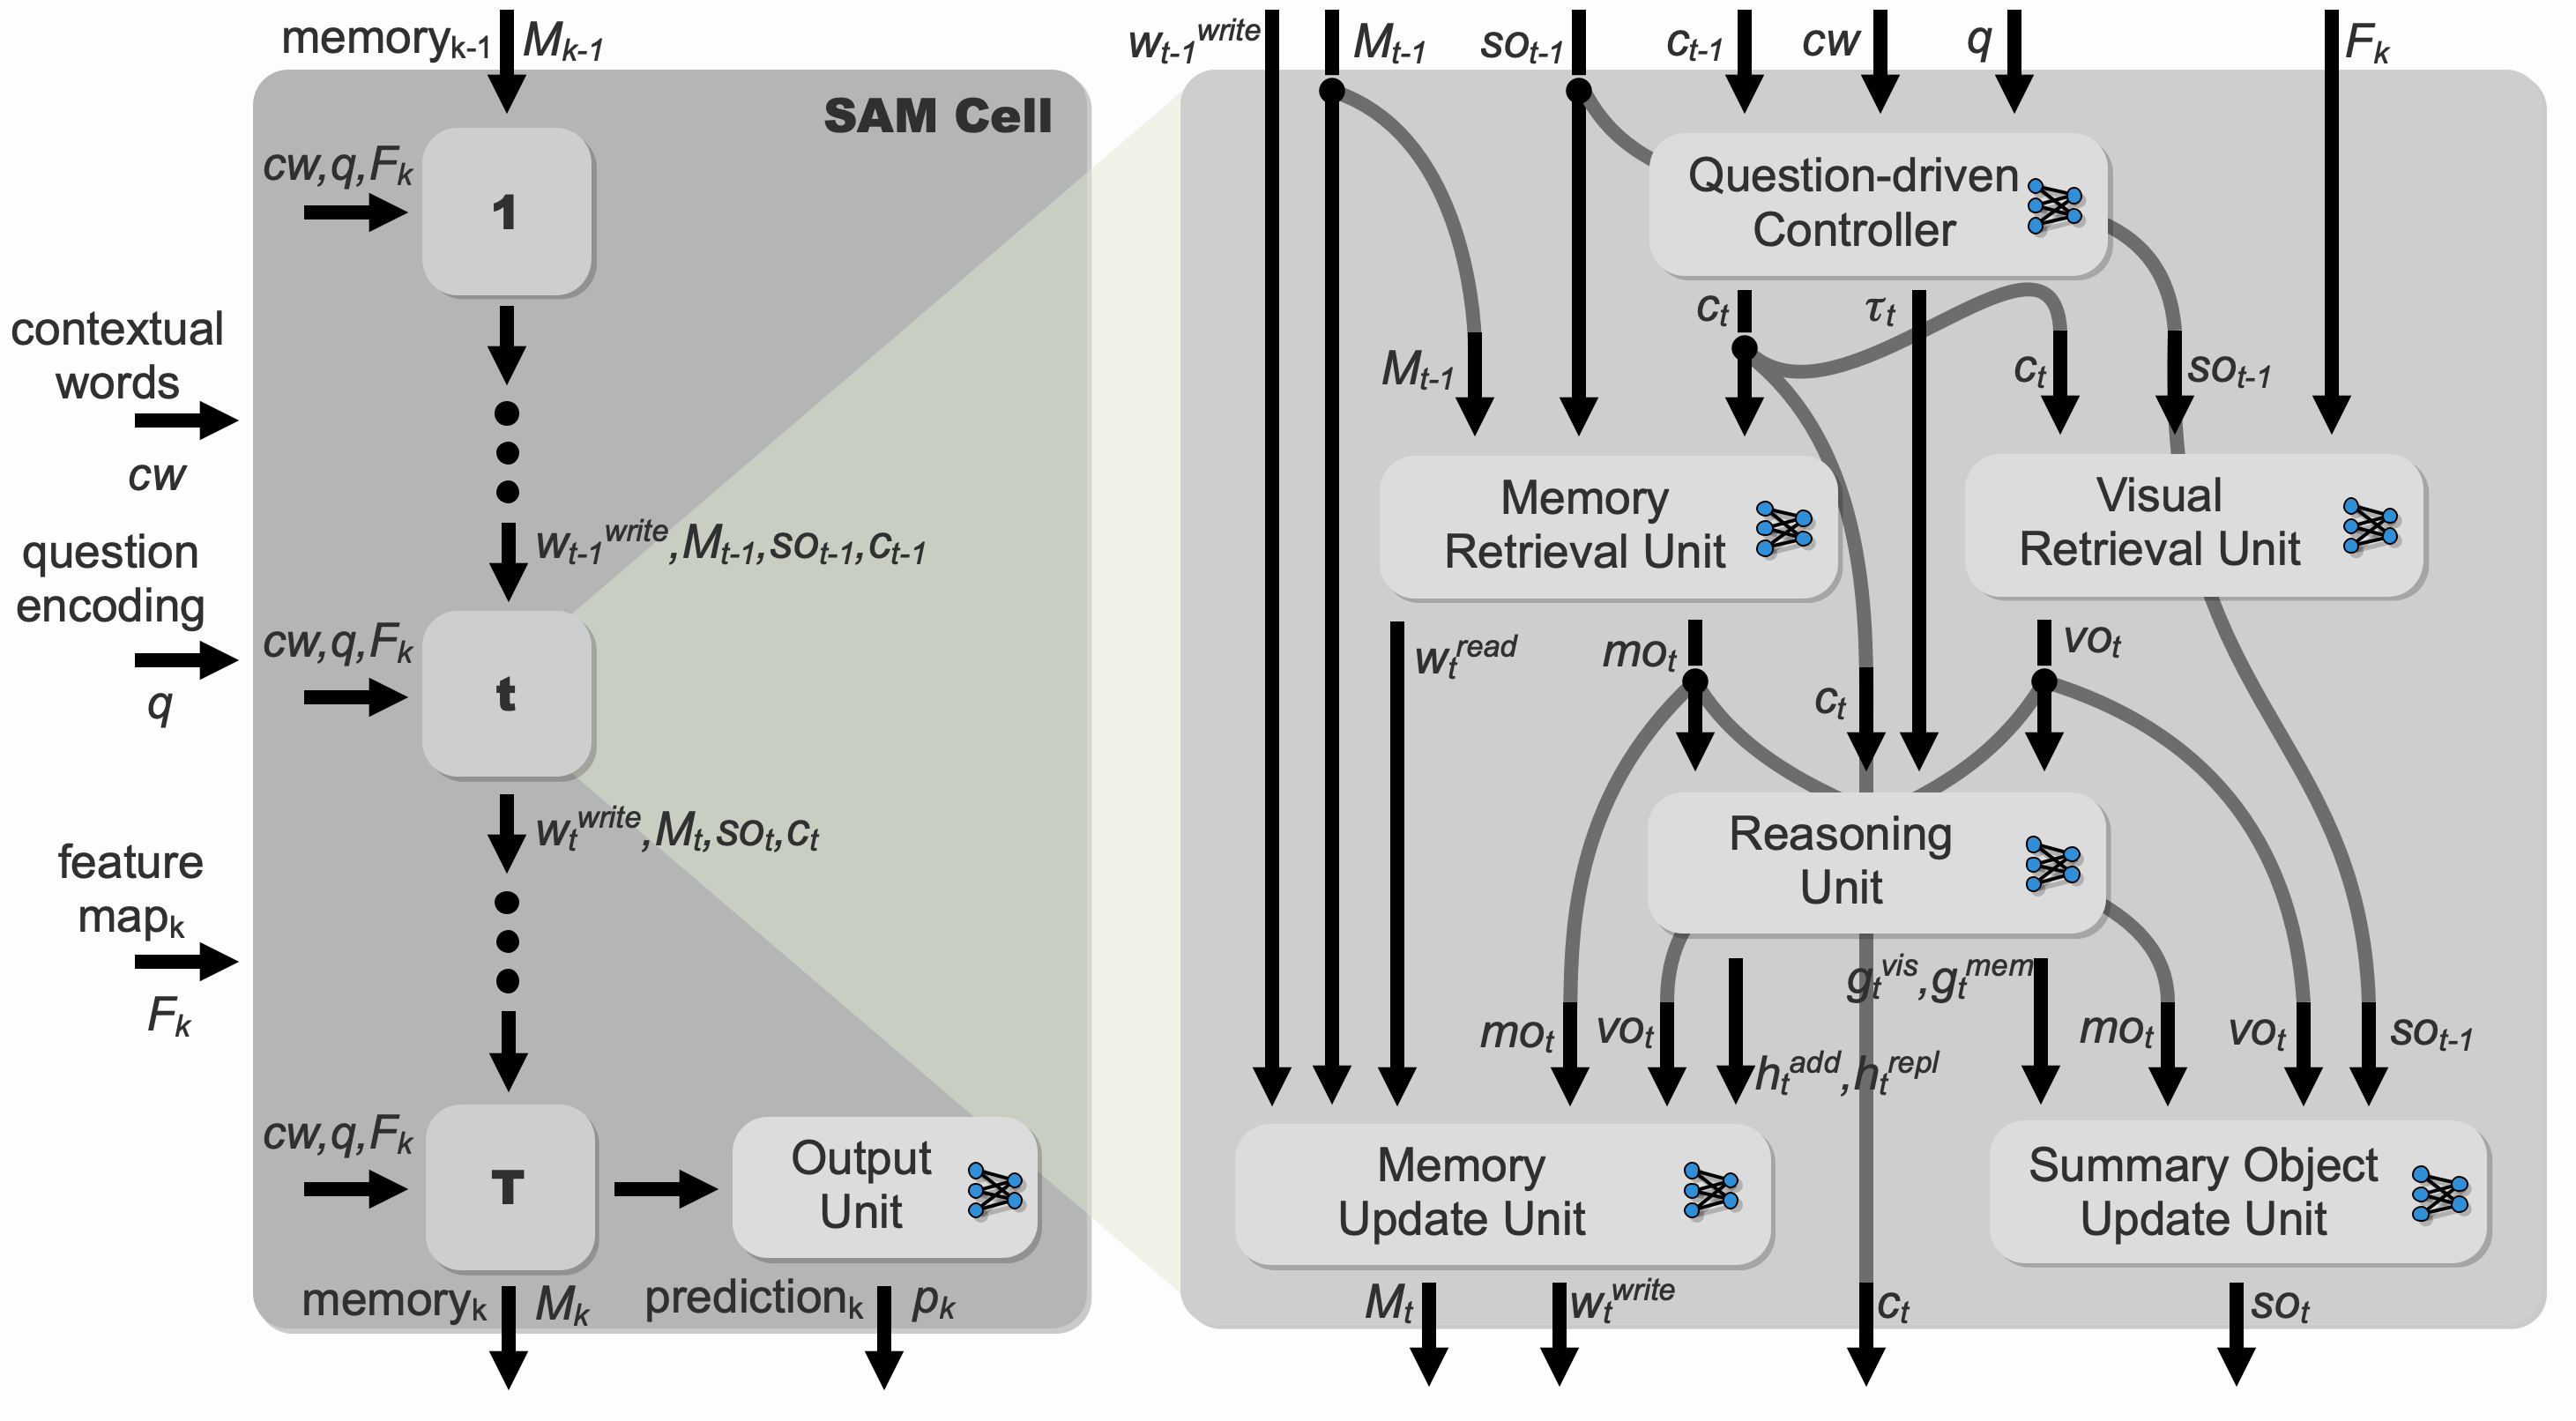
\includegraphics[width=\textwidth]{../img/architecture/samcell_reasoning}
	\caption{Single reasoning step in SAMCell}
	\label{fig:samcell}
\end{figure}	

The core of SAMNet is a recurrent cell called SAMCell (\cref{fig:samcell}). 
By aligning together a new series of $k$ SAMCells per frame, the network can perform $k$ 
reasoning steps over each frame, with information flowing between frames through the external memory. 
While processing a single frame, for $t=1,2, \dots, k$, SAMCell maintains the following information as part of its recurrent state:
(a) $c_t \in \Reals^d$, the control state used to drive the reasoning over objects in the frame and memory; and
(b) $so_t  \in \Reals^d$, the summary visual object representing the relevant object for step $t$.
Let $M_t \in  \Reals^{N \times d}$ denote the external memory with $N$ slots at the end of step $t$.
Let $\whead_t \in  \Reals^N$ denote an attention vector over the memory locations;
in a trained model, $\whead_t$ points to the location of first empty slot in memory for adding new objects.   


This section describes the model and the different units that composed a SAMCell. They are called the Question-driven Controller, the Visual Retrieval Unit, the Memory Retrieval Unit, the Reasoning unit, the Memory update unit, and the Summary Object Udpate Unit. 
The model is also composed of an Image Encoder and a Question Encoder both responsible to pre-process the visual and textual inputs. The output unit is a classifier.
All those modules are described below.














The  Summary Unit is the last unit of the SAMCell. It is responsible to output the new summary object. It first picks which object is relevant between the object extracted from memory and the visual object extracted from the image. Once the relevant object is picked, it is combined with the former summary object through a linear layer to become the new summary object. It is the final step of the SAMCell reasoning cycle. 

The image encoder, question encoder and output unit are described in the appendix.
